\documentclass[UTF8]{ctexrep}

\usepackage{fancyhdr}
\usepackage[letterpaper, left=1in, right=1in, top=1in, bottom=1in]{geometry}
\usepackage{sectsty}
\usepackage{graphicx}
\usepackage{subfig}
\usepackage[section]{placeins}
\usepackage{hyperref}
\usepackage{amsmath}
\usepackage{listings}
\usepackage{color}
\usepackage{lstautogobble}
\usepackage{subfig}

\makeatother
\hypersetup{
    colorlinks=true,
    linkcolor=blue,
    filecolor=magenta,
    urlcolor=cyan,
}
\allsectionsfont{\mdseries\scshape}

\renewcommand{\thesection}{\arabic{section}}

\newcommand{\horrule}[1]{\rule{\linewidth}{#1}}
\title{
    \horrule{0.5pt} \\[0.4cm]
    \huge 2021年第八届中国可视化与可视分析大会\\
    数据可视分析挑战赛\\
    (ChinaVis Data Challenge 2021)\\
    作品说明文档\\
    \horrule{2pt}
}
\author{
    方志成 \ 黄霖 \ 陈雪韬 \ 陈思贝
}
\date{
    % TODO: Date
    2021.6
}
\setcounter{section}{-1}

\begin{document}
    \maketitle

    \section{参赛信息}

    \begin{itemize}
        \item 参赛队名称:上海交通大学—方志成
        \item 作品名称:污染全回顾:2013-2018污染源演化分析与地区污染模式挖掘
        \item 作品主题关键词:污染源分析、污染时空态势分析、污染传输模式分析、大气环境的改善
        \item 团队成员:
        \begin{enumerate}
            \item 方志成,上海交通大学,fangzhicheng@stju.edu.cn,队长
            \item 黄霖,上海交通大学,h1999@stju.edu.cn
            \item 陈雪韬,上海交通大学,xgppt0106@stju.edu.cn
            \item 陈思贝,上海交通大学,tonychen21@stju.edu.cn
            \item 董笑菊,上海交通大学,dong-xj@cs.stju.edu.cn,指导老师
        \end{enumerate}
        \item 团队成员是否与报名表一致:是
        \item 是否学生队:是
        \item 使用的分析工具或开发工具:Express, d3, 高德开放平台
        \item 共计耗费时间(人天):60
        \item 本次比赛结束后,我们是否可以在网络上公布该文档与相关视频:是\\
    \end{itemize}

    \section{作品简介}
    % 请围绕作品主题、要解决的问题\场景、目标用户\读者、应用价值等方面简要介绍作品(建议参赛者描述本部分内容不多于500字,图表不多于1个)
    % TODO: 黄霖

    作品主题以及要解决的问题
    \par
    本作品利用可视分析技术与可视化方法,从时间和空间两个维度展示空气质量大数据背后隐藏的模式和规律,并探索了大气污染的成因和防治方法。
    \par
    本作品的目标用户是需要了解大气污染状况、寻求大气污染治理方法的政府职能部门,以及关切空气质量情况的普通大众。
    \par
    本作品的应用价值,一方面在于为大气污染治理提供帮助,另一方面在于帮助大众认知大气污染的时空态势,唤起人们的环保意识。\\

    \section{数据介绍}
    % 请围绕数据来源、数据格式、数据严谨性、数据清洗等方面简要介绍(建议参赛者描述本部分内容不多于500字,图表不多于3个)
    % TODO: 陈思贝
    % 399 字

    我们的作品使用了竞赛提供的2013–2018年中国高分辨率大气污染再分析开放数据集。该数据集包括了全国42249个观测点的大气气象数据。每个观测点包括了PM2.5、PM10、臭氧、一氧化碳、二氧化硫和二氧化氮等6种常见大气污染物的指数,以及该地当天的平均风速,温湿度等气象信息。我们利用高德开放平台的地理逆编码API,对每一个坐标点经纬度所对应的行政单位进行了映射。对每一个坐标点所述行政区域精确到市(直辖市精确到区)。为配合均值图的展示,本组还对同属同一行政区划的观测点的各污染物数值日均值提前进行了计算。

    同时,我们采用了中华人民共和国生态环境部印发的《国家重点监控企业名单》确认了国家重点监控废水企业、废气企业、污水处理厂、重金属企业和规模化禽畜养殖场的名单。通过高德开放平台的兴趣点查询功能,映射出这些污染源头企业的经纬度和行政区域。并绘制在我们作品的大地图上,与热力图配合使用可以分析不同类型的污染企业与不同大气污染物之间的联系。\\

    \section{分析任务与可视分析总体流程}
    % (建议参赛者描述本部分内容不多于500字,图表不多于3个)
    % TODO: 陈雪韬
    % 309 字
    
    \subsection{分析任务}
    \begin{enumerate}
    	\item 针对 6 项常规污染物,采取合适的方式展现污染物的空间与时间分布态势和变化趋势。
    	\item 针对污染物来源,显示相关污染源信息,方便联系污染源作出对污染物分布模式的分析。
    	\item 针对纬向与经向风速数据,在地图上展现风的大小和方向。
    	\item 针对气温、相对湿度,能够将其作为污染物的辅助分析依据。
    \end{enumerate}

	\subsection{可视分析总体流程}
    本项目将可视化的流程分为两部分:总体分析和局部分析。
    \par
    在总体分析中,项目使用热力图、风向图和两种图的动态展示,从污染物的空间和时间分布上显示了污染物的分布态势,使用污染源分布地图将污染源和污染物的分布相联系分析。
    \par
    在局部分析中,点击任意一地,即可显示该地区的污染物按时间序列分布的均值图,可以通过滑动鼠标滚轮来在不同时间尺度上查看均值图。(图 \ref{fig:analyze_task})
	
	\begin{figure}[h!]
        \centering
        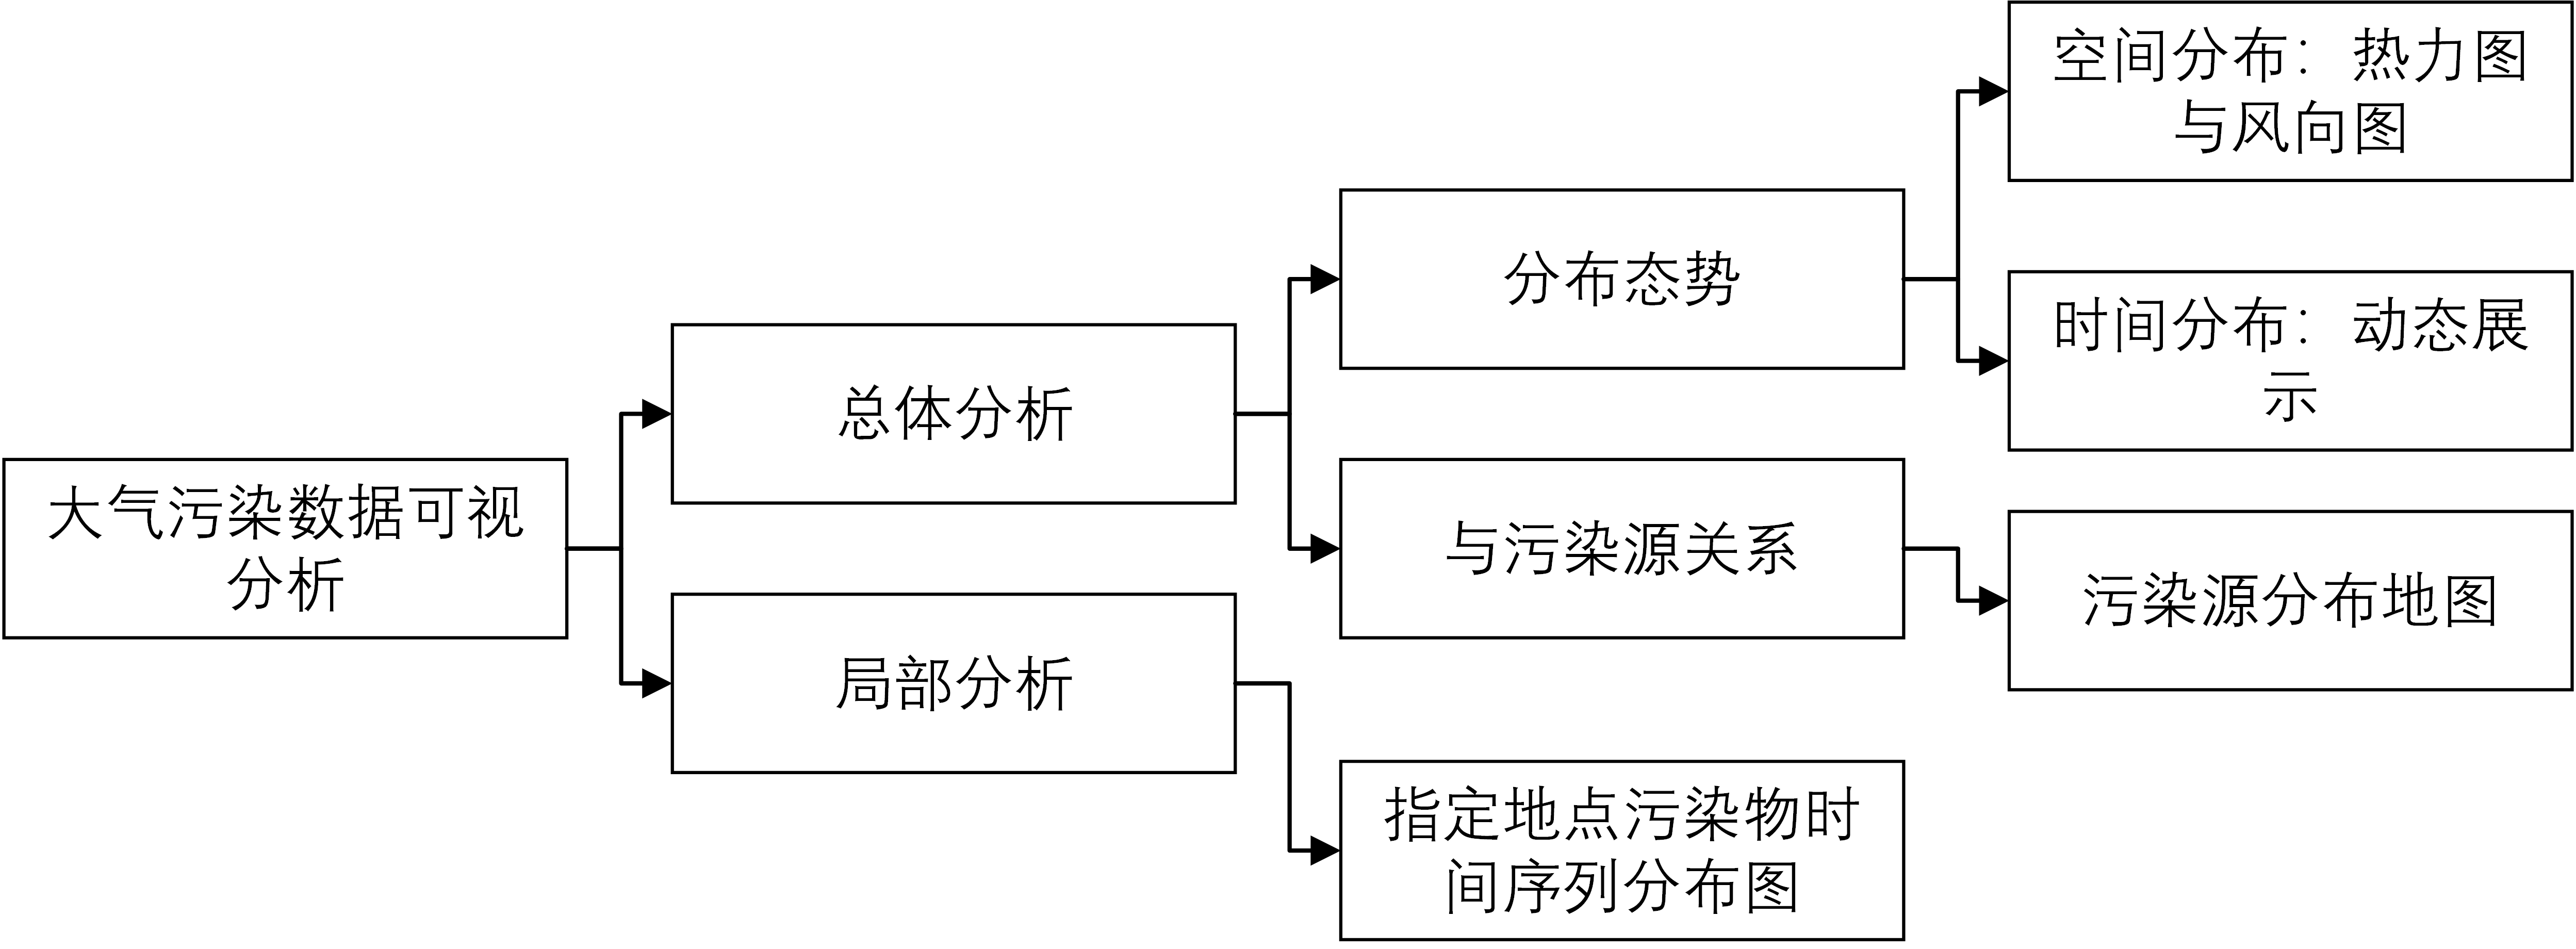
\includegraphics[width=14cm,keepaspectratio]{images/analyze_task.png}
        \caption{分析任务流程图}
        \label{fig:analyze_task}
   	\end{figure}
    	


    \section{数据处理与算法模型}
    % (建议参赛者描述本部分内容不多于1000字,图表不多于5个)
    % TODO: 

    \section{可视化与交互设计}
    % (建议参赛者描述本部分内容不多于1500字,图表不多于5个)

    \subsection{热力图}
	热力图通过高德地图中的heatmap组件实现。用户首先在左边按钮处选择污染指标,再在下边栏目中选定对应的时间,系统会通过SQL语句自动读取对应时间下该污染物指标的数据,并实时地反映到主地图上。而在右侧栏中,用户可以选择显示或隐藏热力图,增加了系统的实用性。
	\par
对于heatmap组件,其可视范围可根据实际效果进行设定;而对于具体的热力点,其半径同样可以根据实际需求进行设定。\\
    

    \subsection{风向图}
	% TODO: 陈雪韬
	% 253 字    
    
	风在地图上以白色的小箭头展示,每个箭头所在处对应一个数据点的风向风速数据。风向通过箭头的指向表示,箭头方向与风向相反;风的大小通过箭头的长度表示,风速与箭头的长度成正比关系。
    
	\begin{figure}[h!]
        \centering
        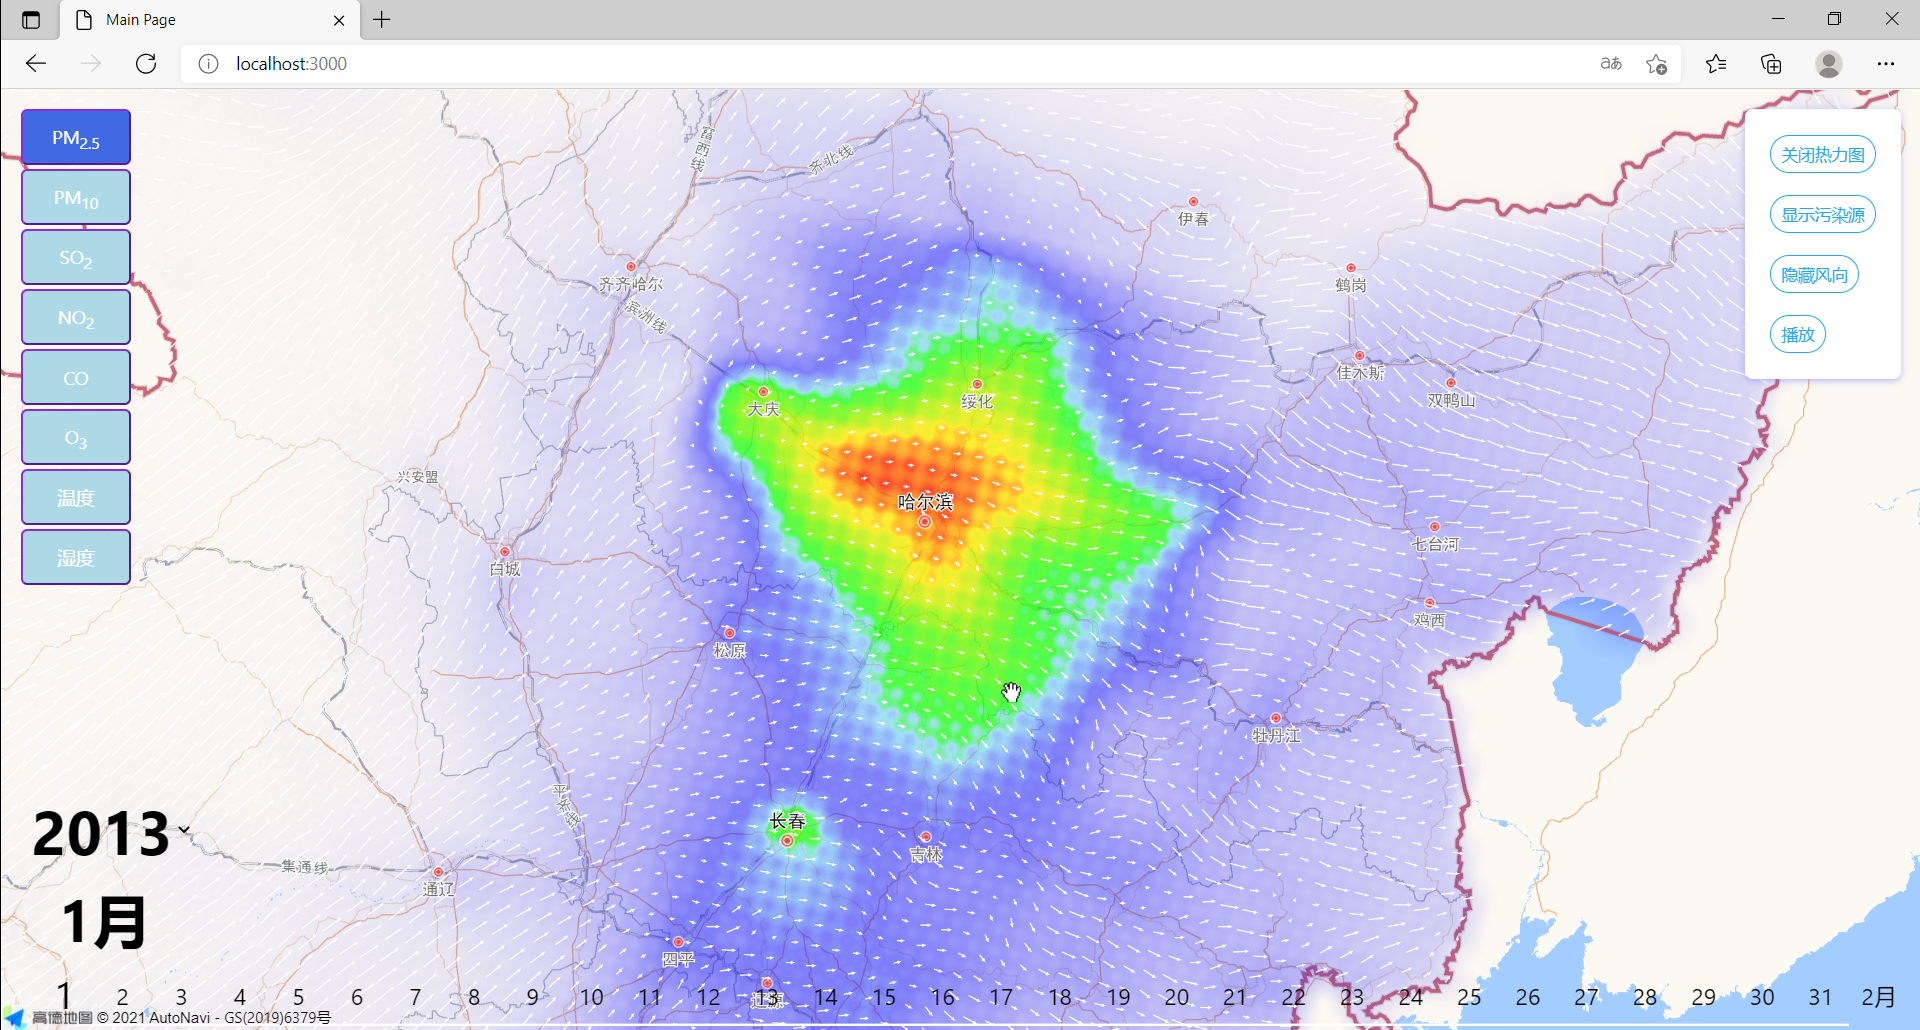
\includegraphics[width=15cm,keepaspectratio]{images/wind_map1.png}
        \caption{哈尔滨 1 日污染物热力与风向图}
        \label{fig:wind_map1}
    \end{figure}
    
    我们可以通过风向图和污染物热力图来查看风对污染物扩散造成的影响。如图 \ref{fig:wind_map1} ,哈尔滨 1 日风向图中所示,哈尔滨该天 $\mathrm{PM}_{2.5}$ 污染浓度积聚较高,这与哈尔滨该天的风有关:该天风速并不是很大,风向也较为紊乱无序,所以可以判断污染物在该地还会停留较多的时间;与此相比,在哈尔滨 2 日风向图与污染物热力图(图 \ref{fig:wind_map2})中,哈尔滨迎来了西北风,整体的 $\mathrm{PM}_{2.5}$ 污染物向东南方向扩散。\\
    
    \begin{figure}[h!]
        \centering
        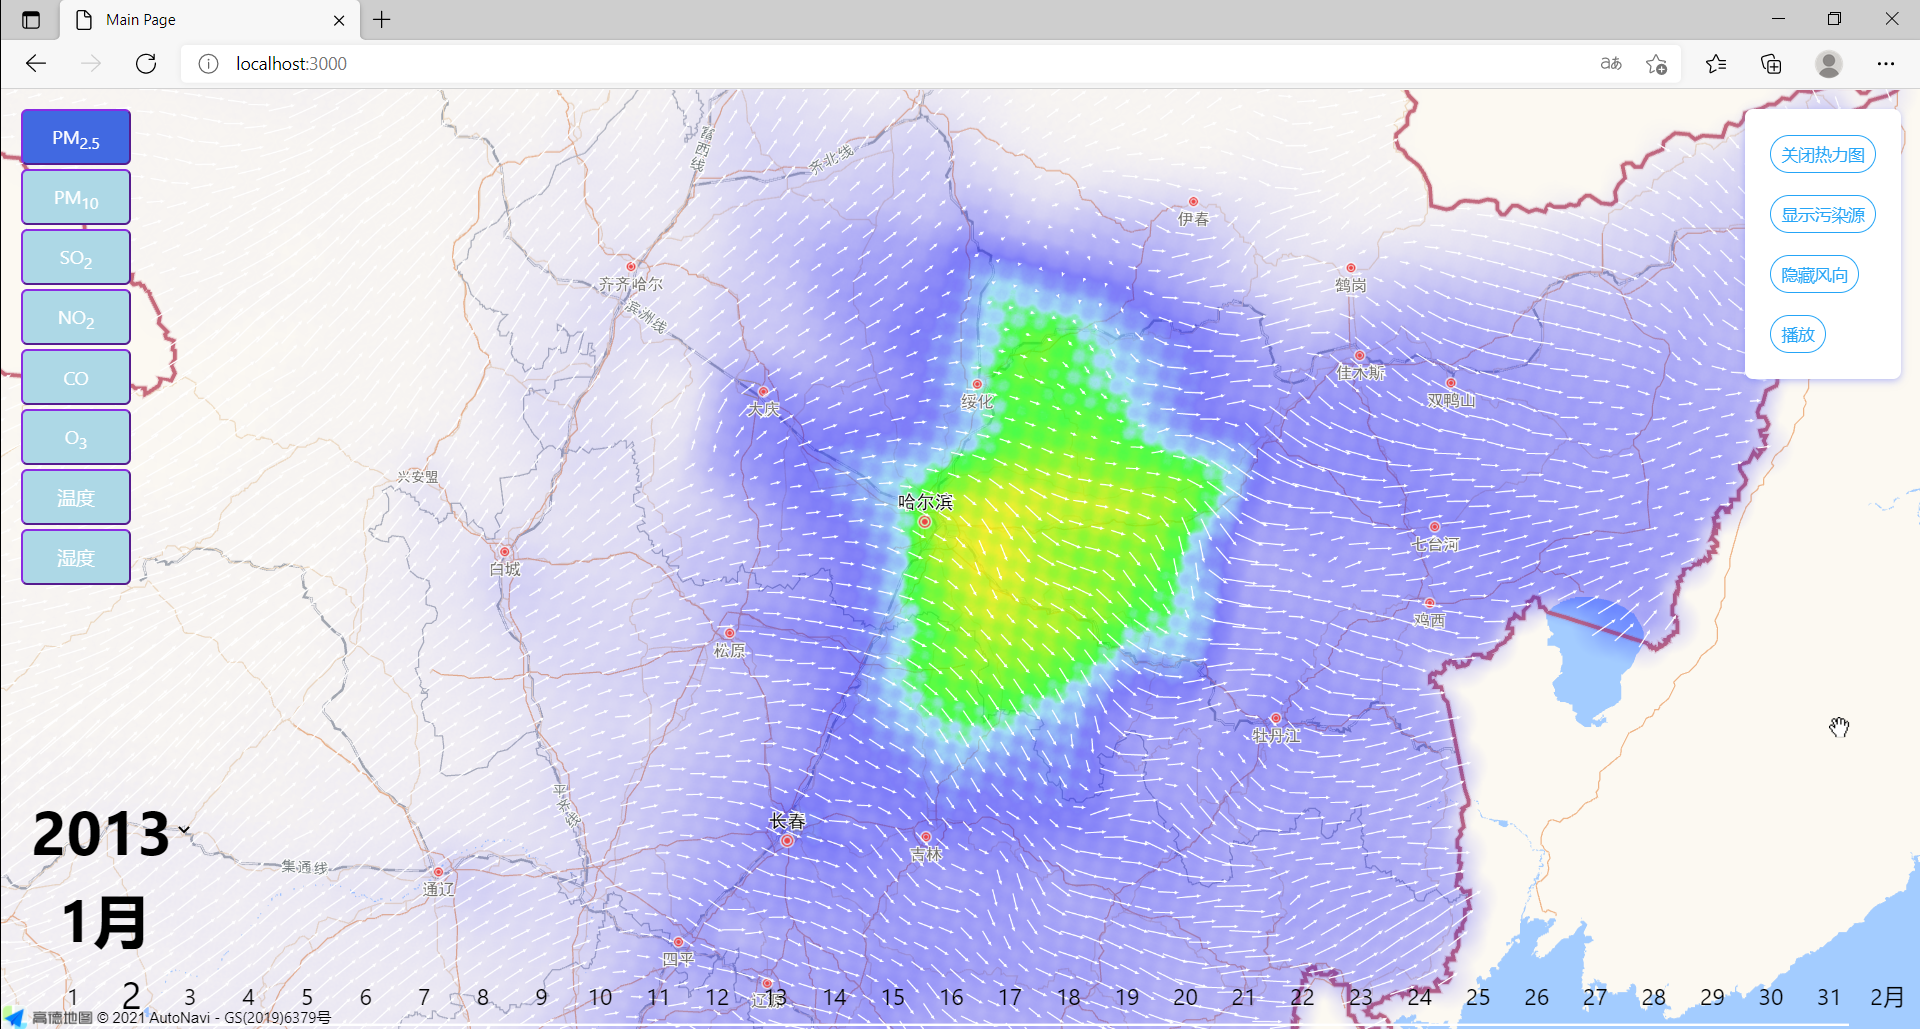
\includegraphics[width=15cm,keepaspectratio]{images/wind_map2.png}
        \caption{哈尔滨 2 日污染物热力与风向图}
        \label{fig:wind_map2}
    \end{figure}


    \subsection{污染源}
    % TODO: 陈思贝
    % 282字

    污染源头的信息以标志的形式在地图模块上展示。针对不同类型的污染企业,采用了不同的图标和颜色以进行区分(见图 \ref{fig:pollution_source_demo1})。为便于可视化展示污染源信息,我们为展示污染源的功能添加了展示和隐藏的按钮。与热力图叠加展示时,可以清晰看出污染源企业密集的区域与大气污染严重的区域存在高度的重合。我们对污染源信息的展示设置了缩放限制,当地图缩小到一定比例时,会隐藏图标以避免图标过于密集降低了视图的可读性。当鼠标悬浮于某一污染企业的图标上时,还会展示该企业名称等相关信息。选择显示污染源后,在地图右上角会展示污染源的图例。图例旁的复选框可用于隐藏部分类型的污染企业,筛选出感兴趣的数据。\\

    \begin{figure}[h!]
        \centering
        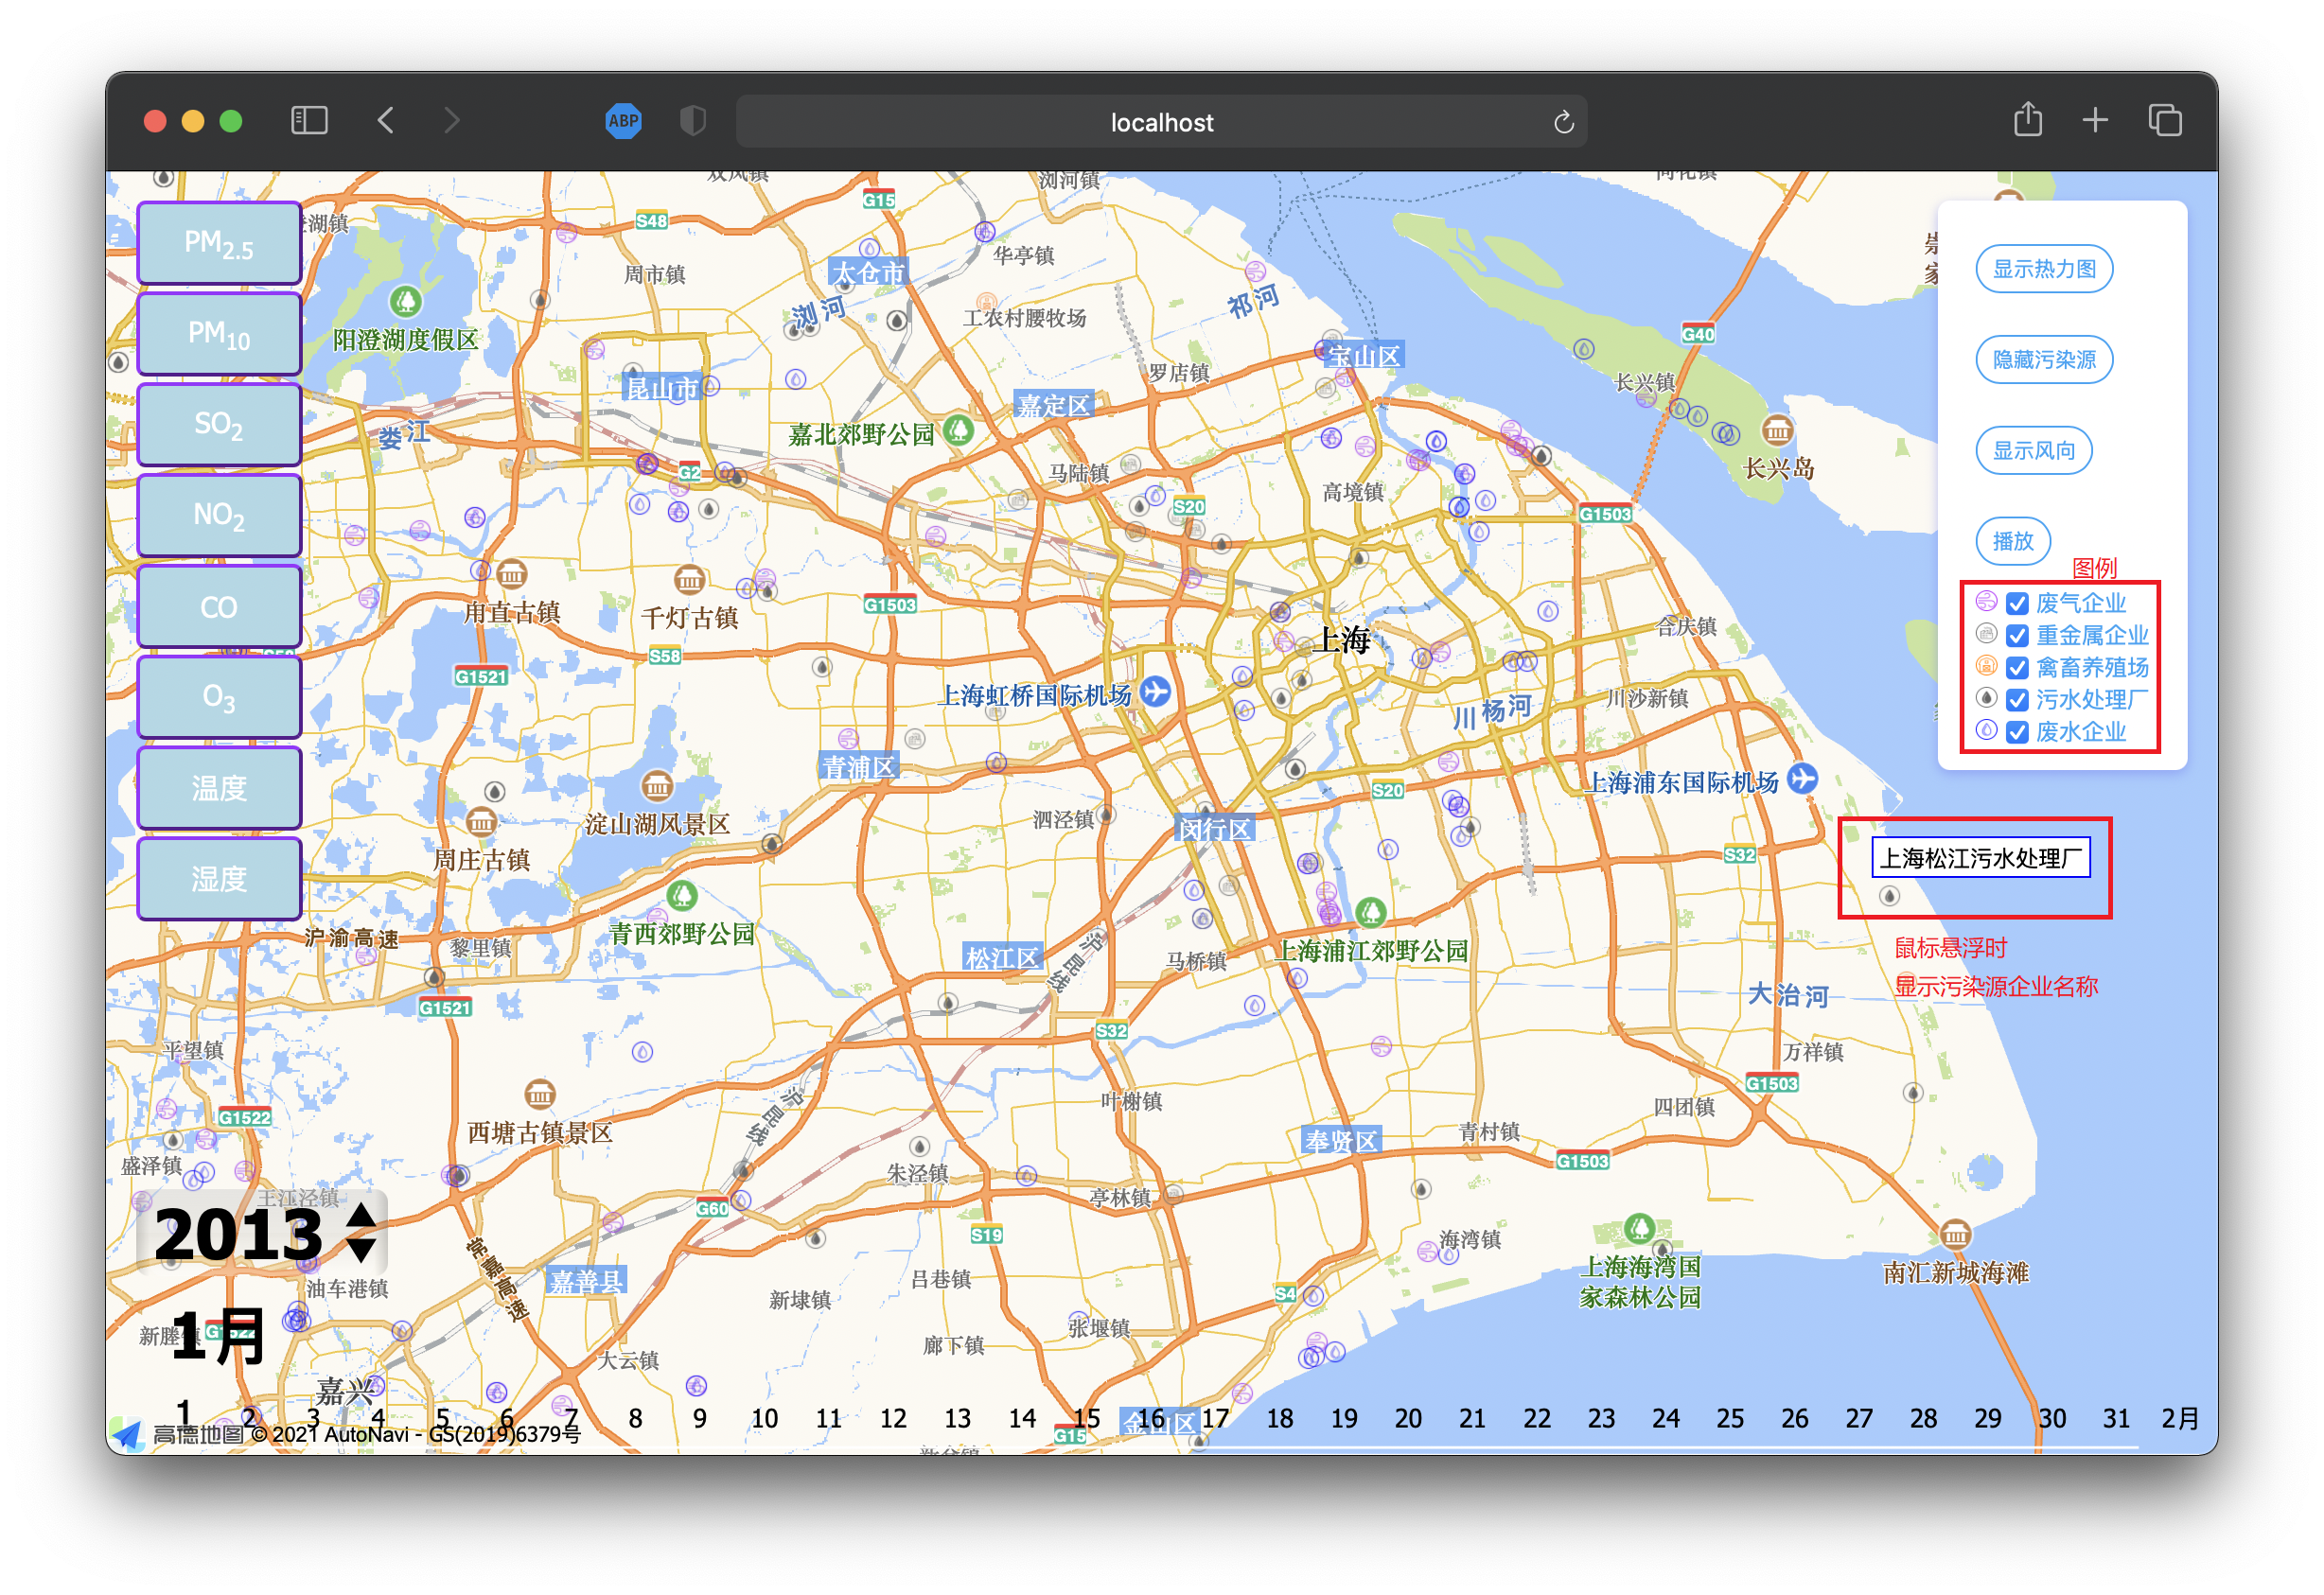
\includegraphics[width=15cm,keepaspectratio]{images/pollution_source_demo1.png}
        \caption{显示污染源功能展示}
        \label{fig:pollution_source_demo1}
    \end{figure}

    \subsection{均值图}
    用户在地图中选取城市,在左上角污染物菜单选取污染类型,之后均值图会自动绘制。
    \par
    均值图的横轴是时间,可以在合适范围内任意缩放、拖动,纵轴是污染物浓度,颜色会随污染程度的严重而加深。
    利用均值图可以观察当地的空气污染程度随时间的演变。
    \par
    均值图同时也作为热力图的时间选取控件,用户在均值图中依次选取年、月、日来更新热力图对应的时间。
    均值图作为时间的选取控件,也支持自动播放,动态展示出污染物浓度随时间的变化。
    \par

    \section{实验、案例与场景分析}
    % (建议参赛者描述本部分内容不多于2000字,图表不多于10个)

    \subsection{大气污染源分析}
    % 利用可视分析技术,识别主要大气污染源,分析关键污染成因。(可以根据自身情况联合其他数据辅助分析)
    % TODO: 陈思贝
    % 532 字

    通过叠加热力图与重点监控污染企业,我们可以识别出主要大气污染物与污染企业之间的联系。尽管公众普遍认为发电厂、炼钢厂这一类的企业对大气污染有着极大的共享,但图表分析显示主要大气污染源与人们日常生活息息相关。以2013年4月12日长三角及周边大型城市的热力图为例(见图\ref{fig:source_city}),除臭氧外的各项污染物指标均在上海、长沙、武汉等大型城市附近最为严重。而在大型工厂聚集的空旷地区,大气污染物指数却并无明显上升。

    这些大气污染物来源与居民生活息息相关,汽车尾气贡献了绝大部分的大气污染物。以二氧化氮为例,其主要来自燃料燃烧与汽车尾气。图\ref{fig:source_city}中武汉市周围的二氧化氮指数明显过高,其范围与颜色深度均可与上海市匹敌。但其他大气污染物却没有显著上升。经过分析可能与武汉市未实行小轿车限制上牌措施有关,长三角区域全部主要城市都实施了汽油车限制上牌的措施,因此无限牌措施的武汉市二氧化氮指数偏高。

    臭氧指数与其他主要大气污染指数呈现出的趋势大相径庭。其整体分布较为平衡,并不存在局部臭氧指数过高的现象。尽管处于平流层的臭氧被称为有益处的臭氧层,但处于地表对流层的臭氧会对人类产生影响。地表的臭氧层主要由阳光分解形成,因此从图\ref{fig:o3_tibet}中可以看出青藏高原地区海拔高,阳光更加充足,尽管人类活动较小,其臭氧浓度也更高。


    \begin{figure}[h!]
        \centering
        \subfloat[$\mathrm{PM}_{2.5}$热力图]{\includegraphics[width=0.3\columnwidth]{images/source_pm25.png}}
        \subfloat[$\mathrm{PM}_{10}$热力图]{\includegraphics[width=0.3\columnwidth]{images/source_pm10.png}}
        \subfloat[二氧化硫热力图]{\includegraphics[width=0.3\columnwidth]{images/source_so2.png}}\\
        \subfloat[二氧化氮热力图]{\includegraphics[width=0.3\columnwidth]{images/source_no2.png}}
        \subfloat[一氧化碳热力图]{\includegraphics[width=0.3\columnwidth]{images/source_co.png}}
        \subfloat[臭氧热力图]{\includegraphics[width=0.3\columnwidth]{images/source_o3.png}}
        \caption{长三角区域大气污染物热力图}
        \label{fig:source_city}
    \end{figure}

    \begin{figure}[h!]
        \centering
        \includegraphics[width=10cm,keepaspectratio]{images/o3_demo.png}
        \caption{青藏高原地区臭氧浓度热力图}
        \label{fig:o3_tibet}
    \end{figure}

    \subsection{大气污染时空态势分析}
    % 利用可视分析技术,分析大气污染时空分布模式、监控大气污染时空演变态势。
    % TODO: 方志成
    通过本项目提供的“播放”功能,能够实现热力图与风向图随时间而变化的动态展示。以浙江地区2013的部分月份为例,如图所示,浙江省2013年5月至7月的$\mathrm{PM}_{10}$污染浓度呈现了一个从南向北的趋势;而结合风向图可以发现,这三个月以南风为主,结合$\mathrm{PM}_{10}$颗粒较大等因素,推断出局部的$\mathrm{PM}_{10}$颗粒污染受风向影响随时间出现了北移的现象。并且,通过2014年类似的情况,验证了分析得到的结论。
    
    \begin{figure}[h!]
        \centering
        \subfloat[2013年1月5日热力图]{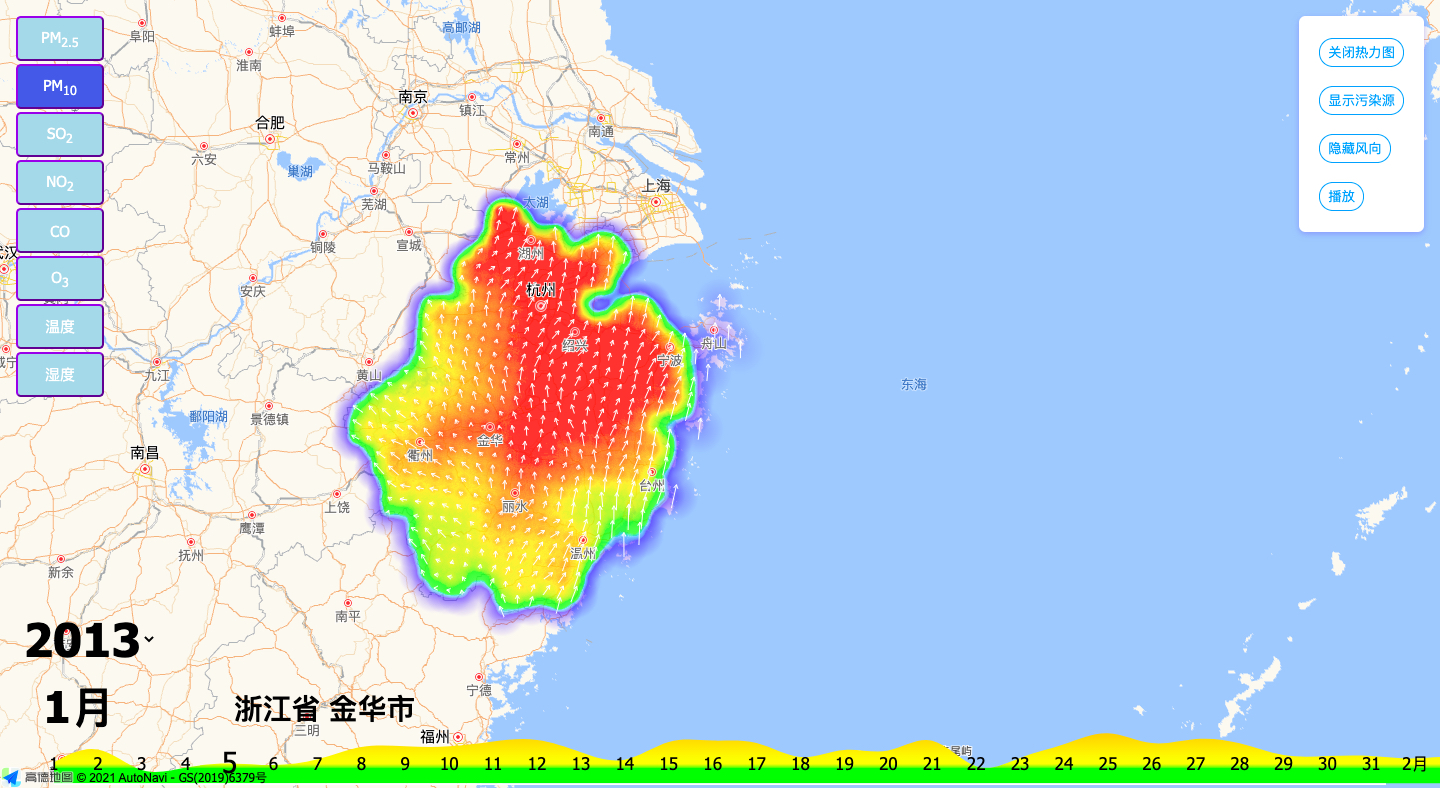
\includegraphics[width=0.3\columnwidth]{images/time_space1.png}}
        \subfloat[2013年1月6日热力图]{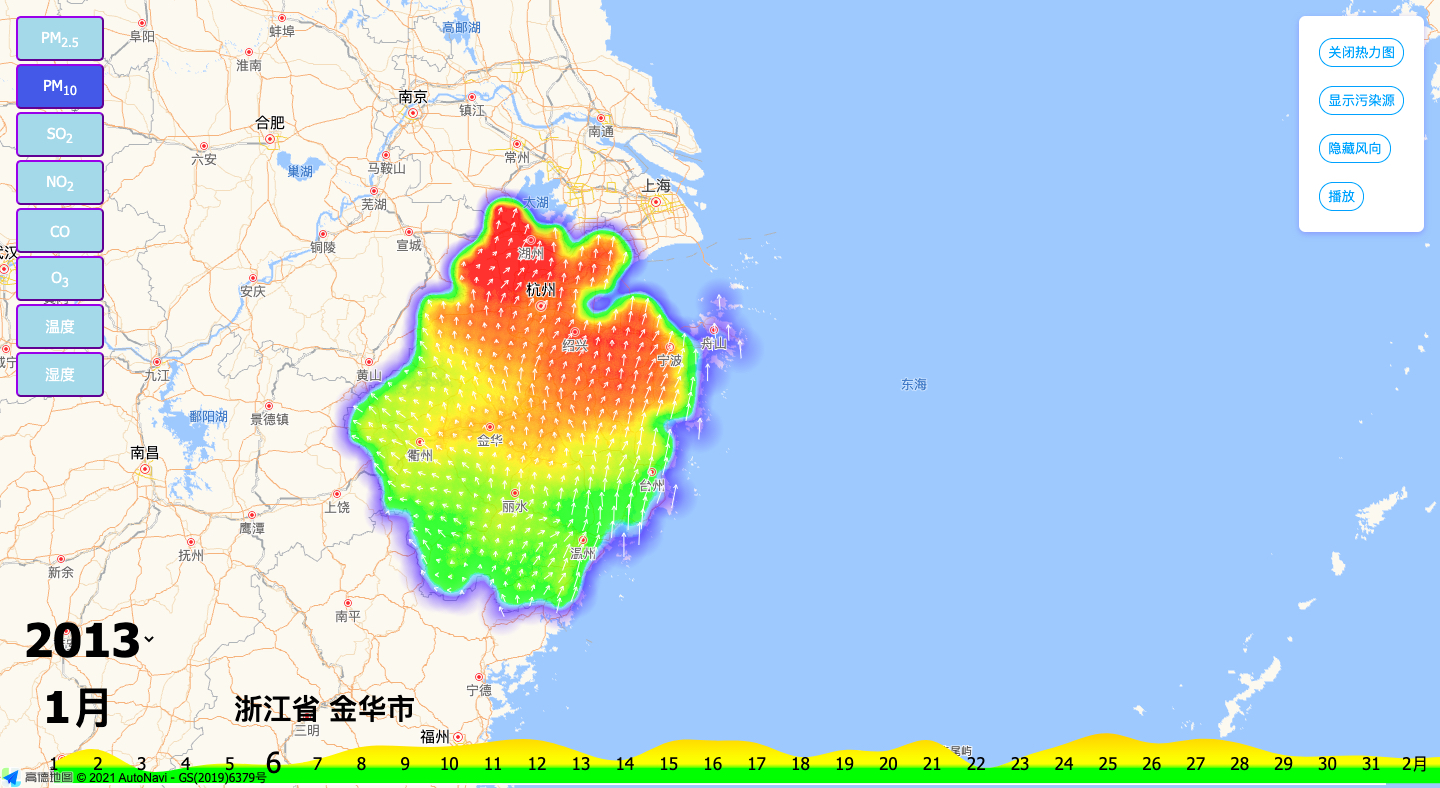
\includegraphics[width=0.3\columnwidth]{images/time_space2.png}}
        \subfloat[2013年1月7日热力图]{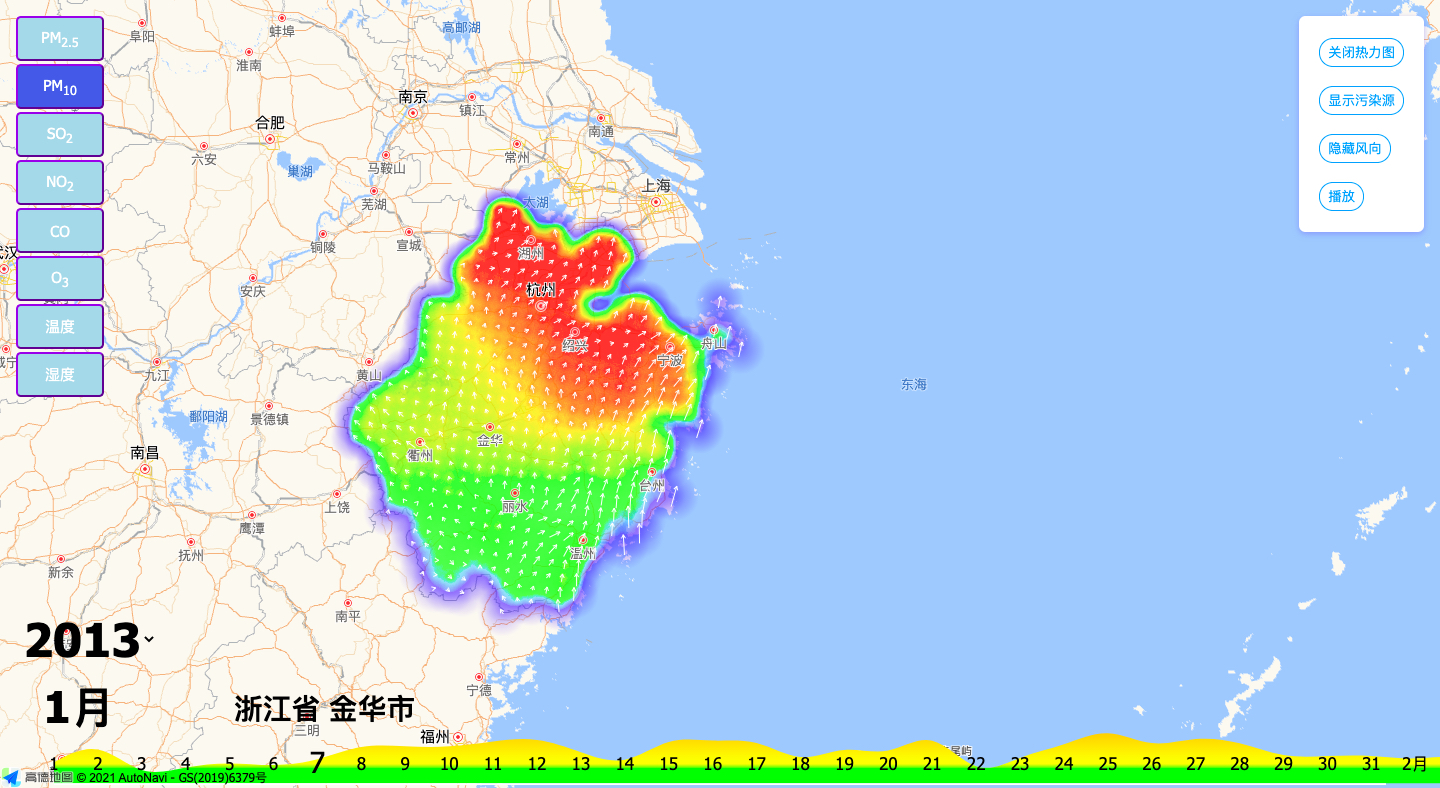
\includegraphics[width=0.3\columnwidth]{images/time_space3.png}} \\
        \subfloat[2014年1月5日热力图]{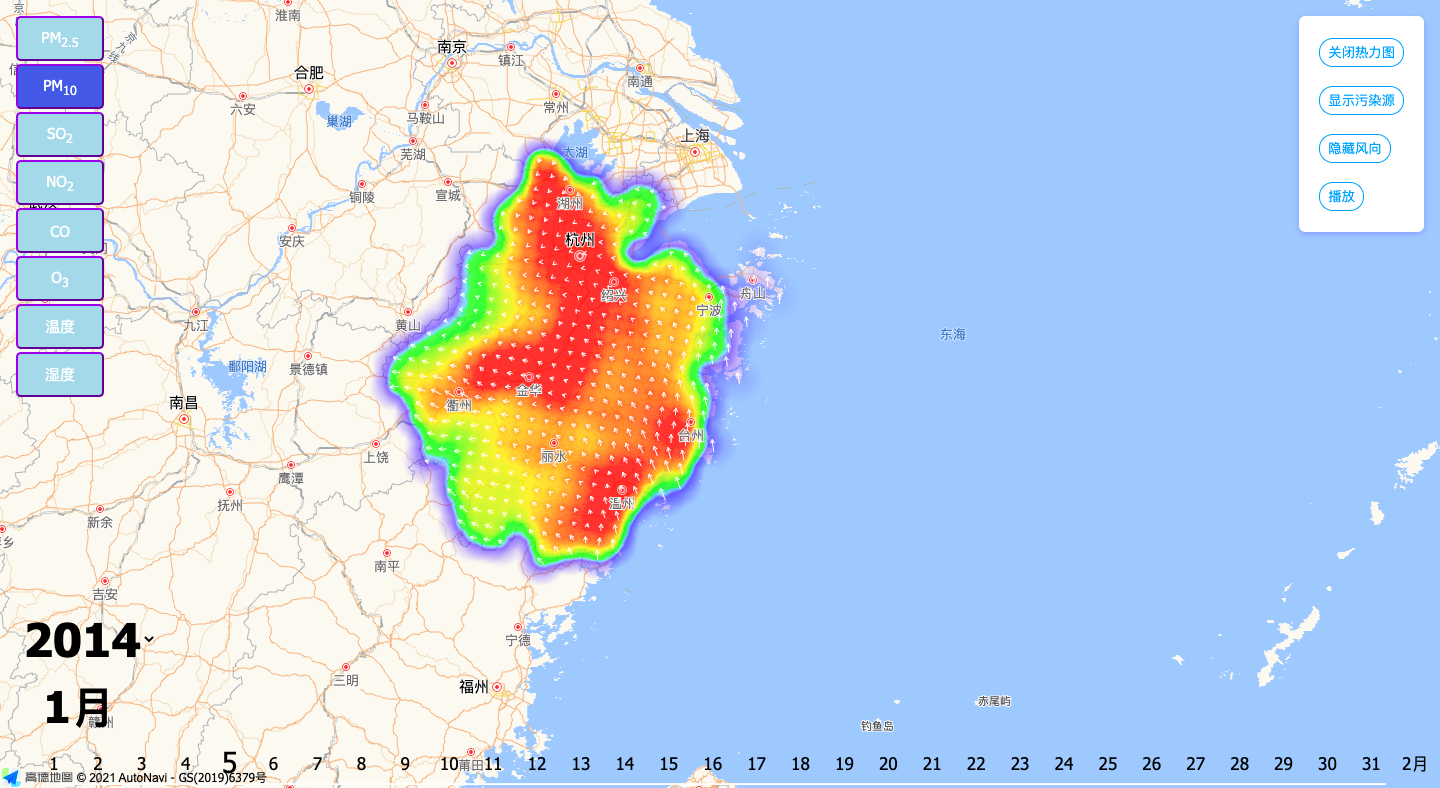
\includegraphics[width=0.3\columnwidth]{images/time_space4.png}}
        \subfloat[2014年1月6日热力图]{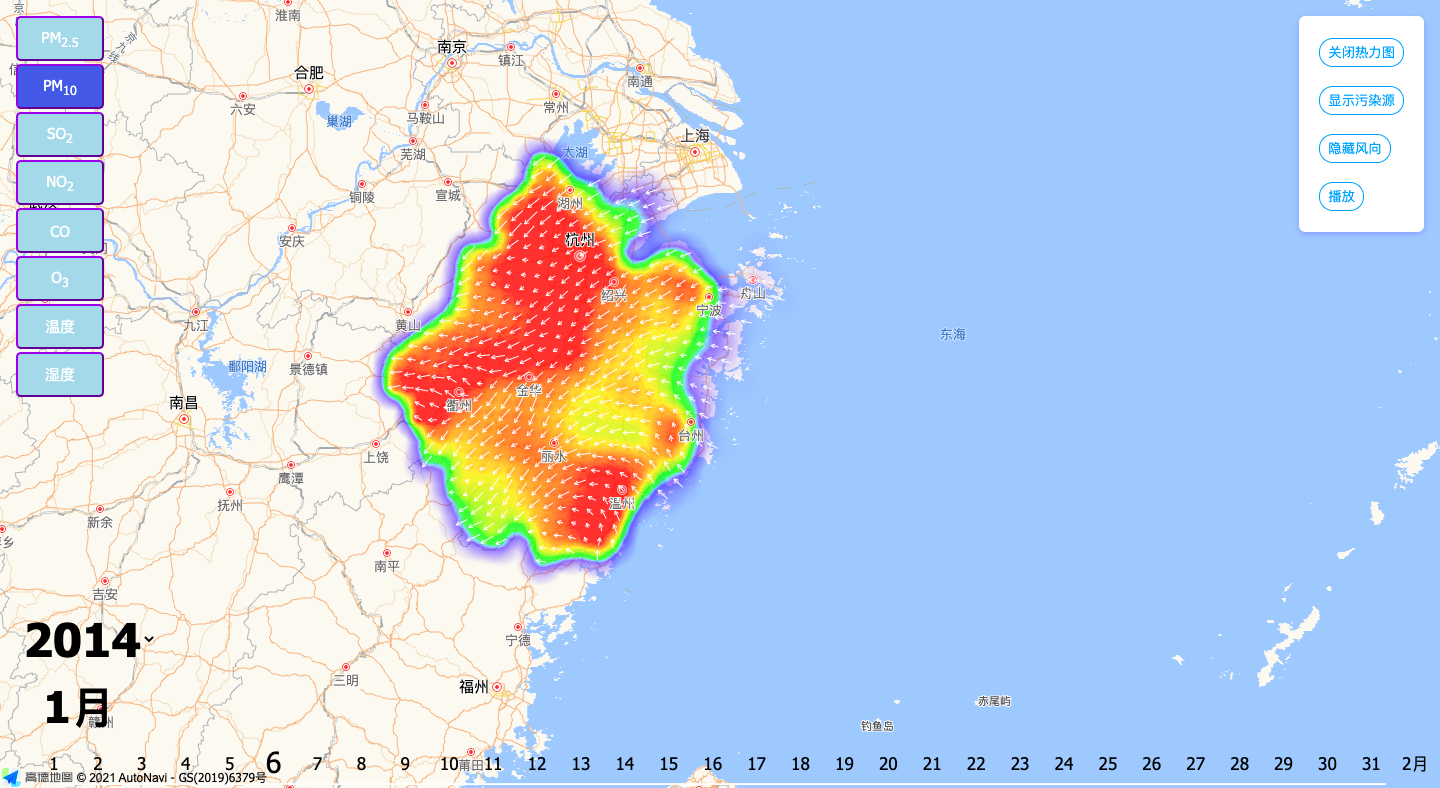
\includegraphics[width=0.3\columnwidth]{images/time_space5.png}}
        \subfloat[2014年1月7日热力图]{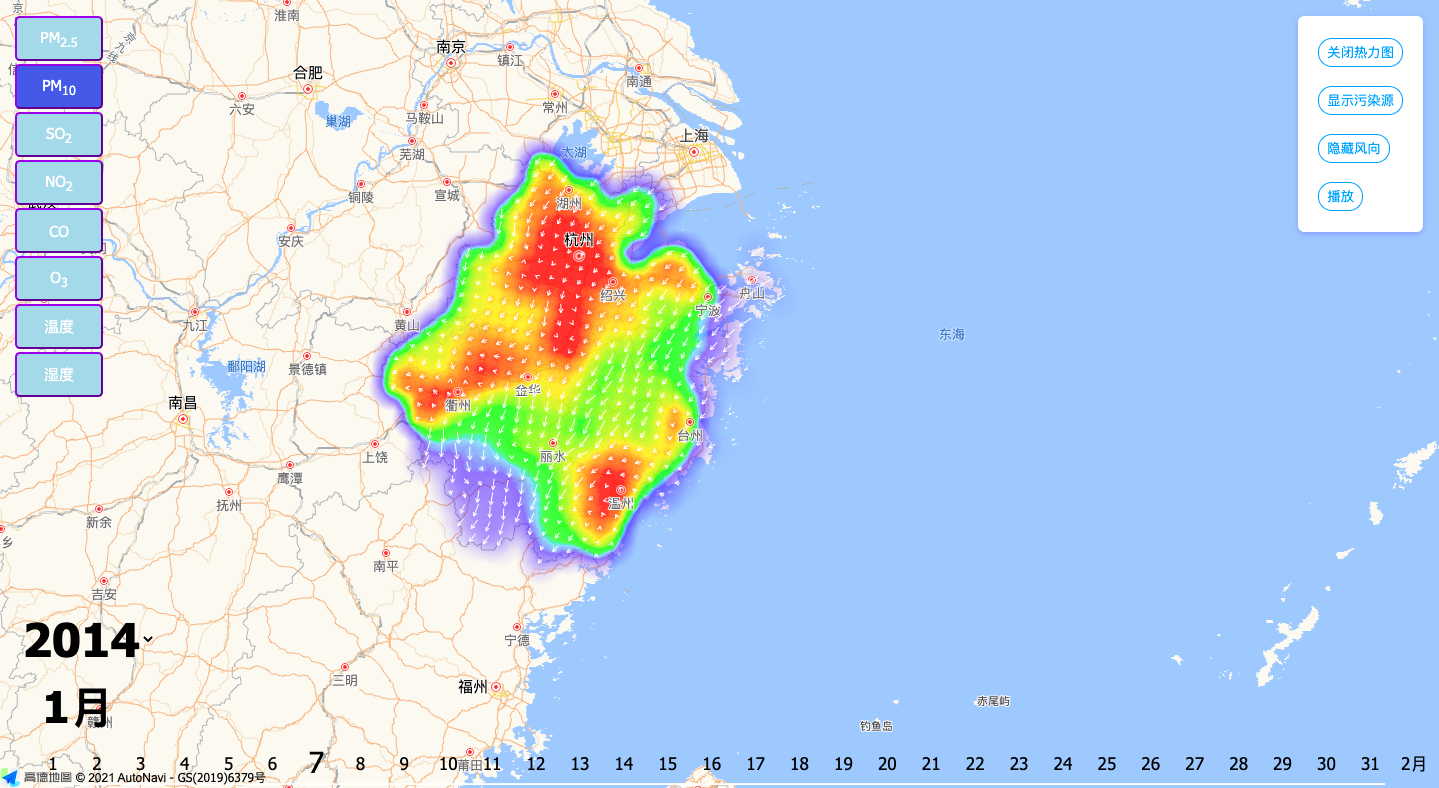
\includegraphics[width=0.3\columnwidth]{images/time_space6.png}}
        \caption{浙江省$\mathrm{PM}_{10}$污染局部热力图}
        \label{fig:time_space1}
    \end{figure}
    
    \begin{figure}[h!]
        \centering
        \subfloat[2017年1月$\mathrm{O}_{3}$热力图]{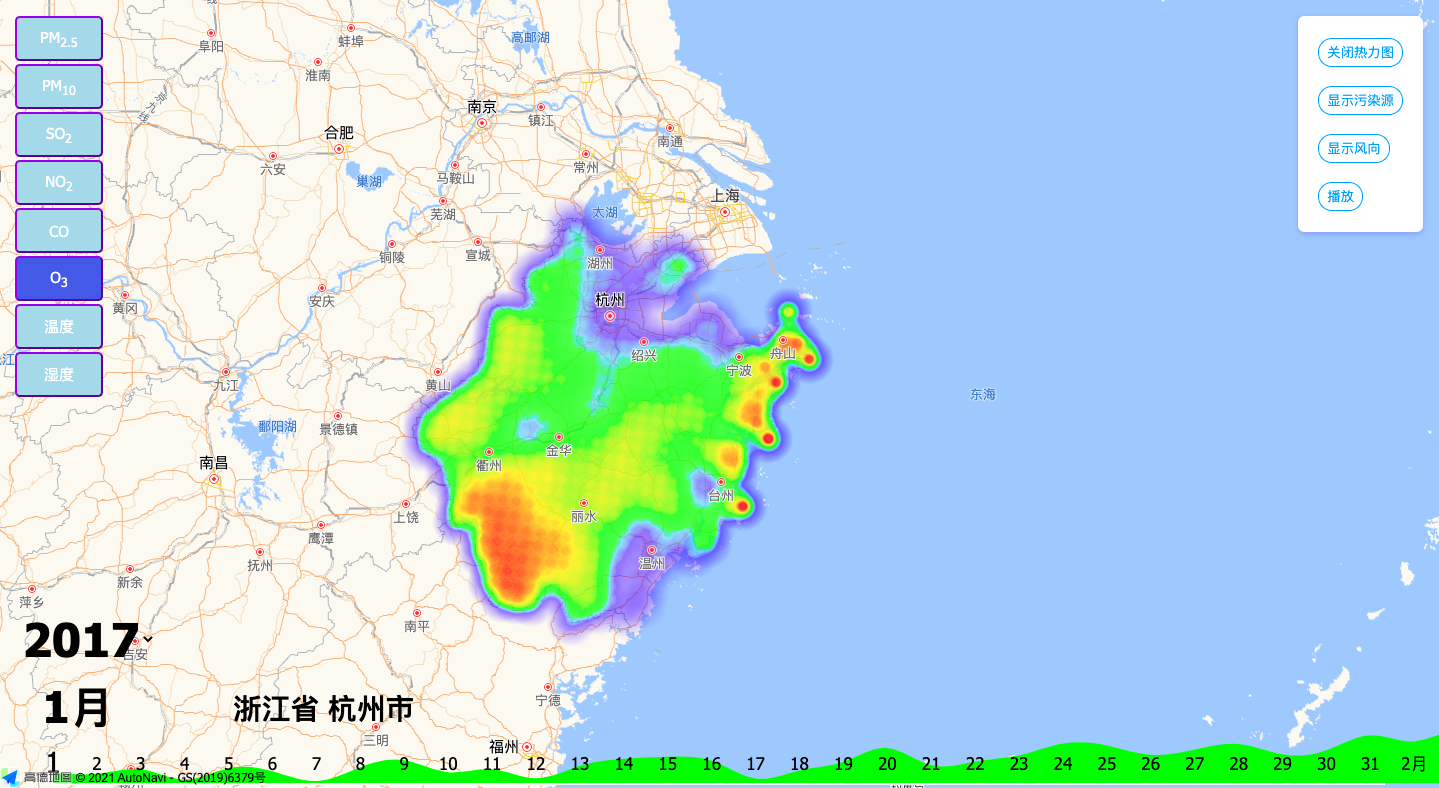
\includegraphics[width=0.5\columnwidth]{images/time_space7.png}}
        \subfloat[2017年6月$\mathrm{O}_{3}$热力图]{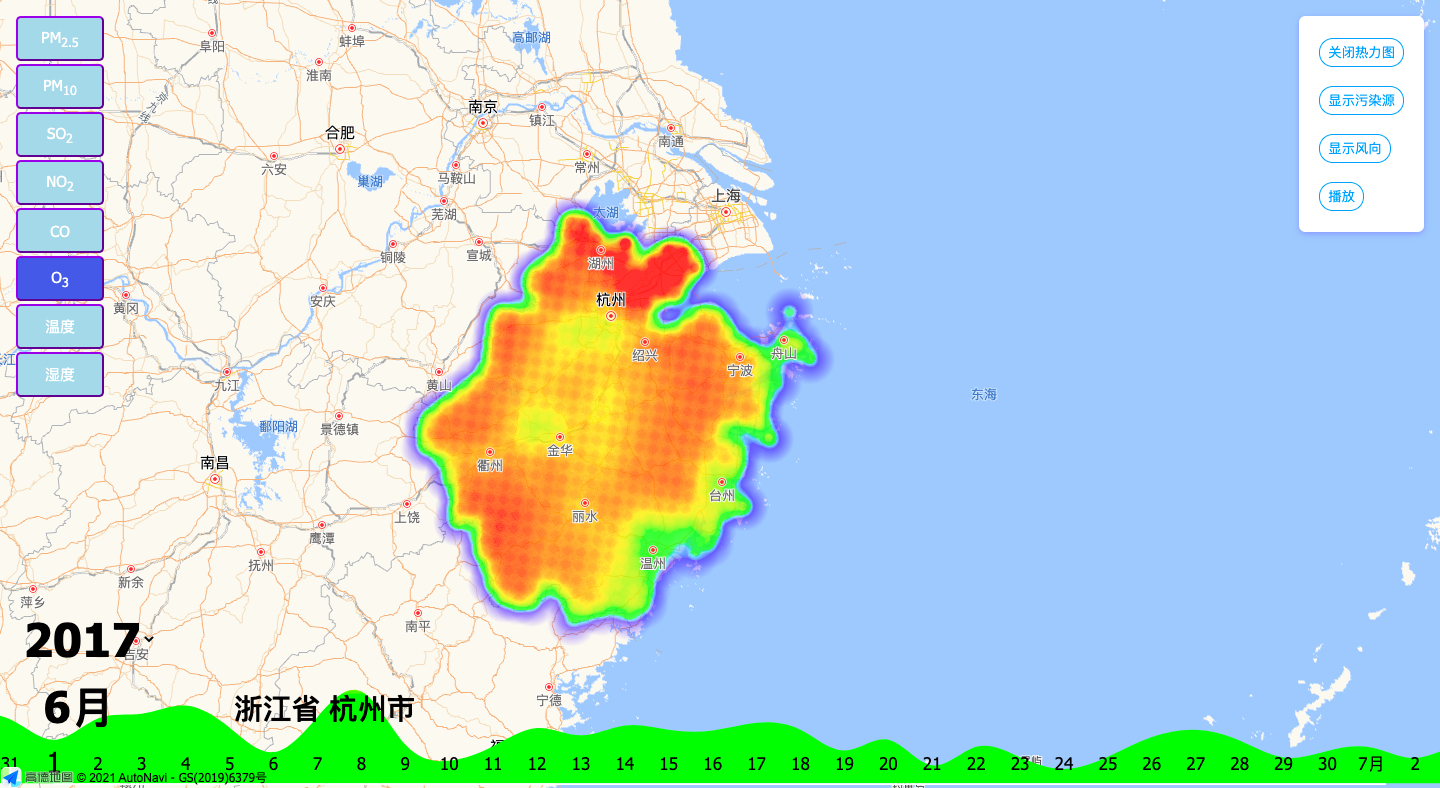
\includegraphics[width=0.5\columnwidth]{images/time_space8.png}} \\
        \subfloat[2013年4月$\mathrm{SO}_{2}$热力图]{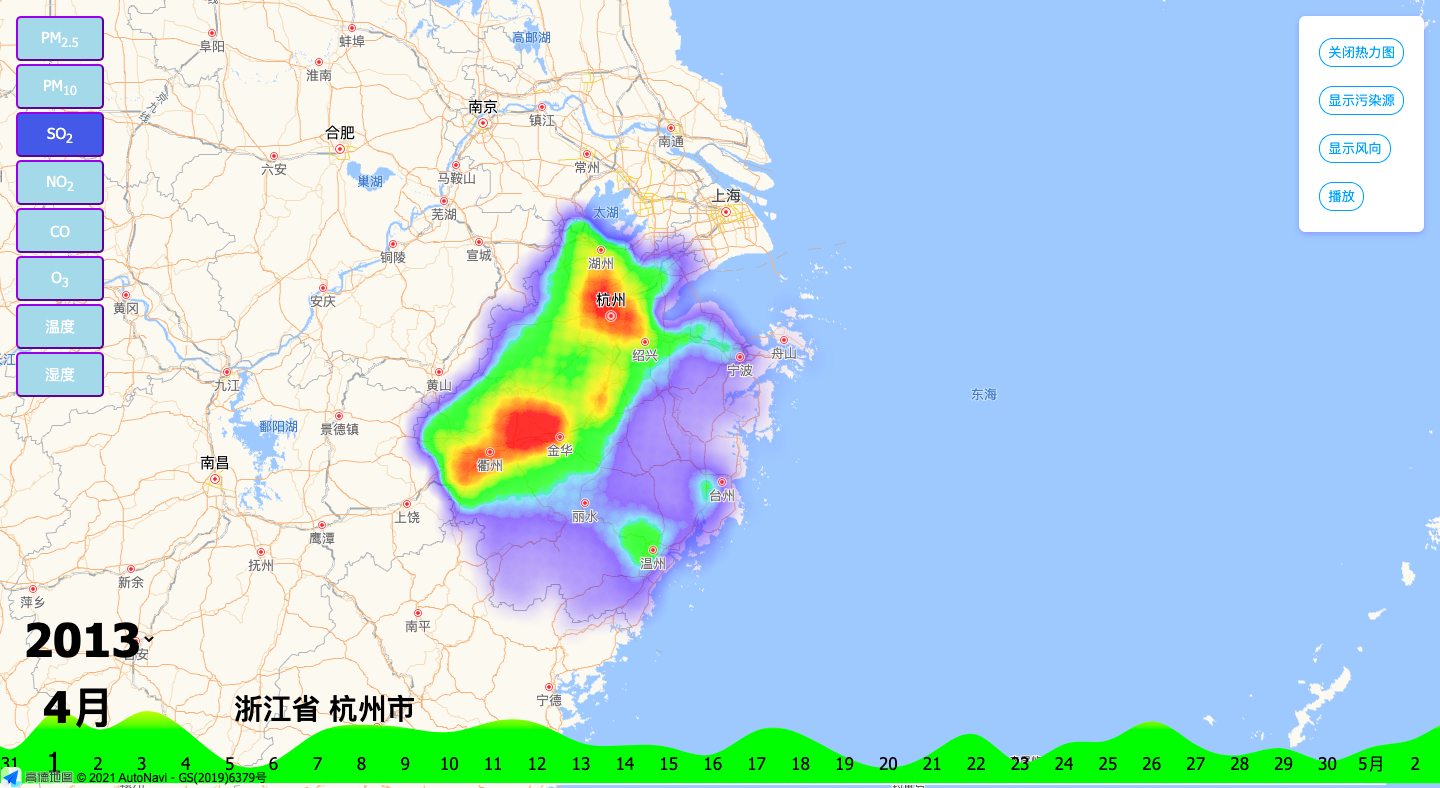
\includegraphics[width=0.5\columnwidth]{images/time_space9.png}} 
        \subfloat[2015年4月$\mathrm{SO}_{2}$热力图]{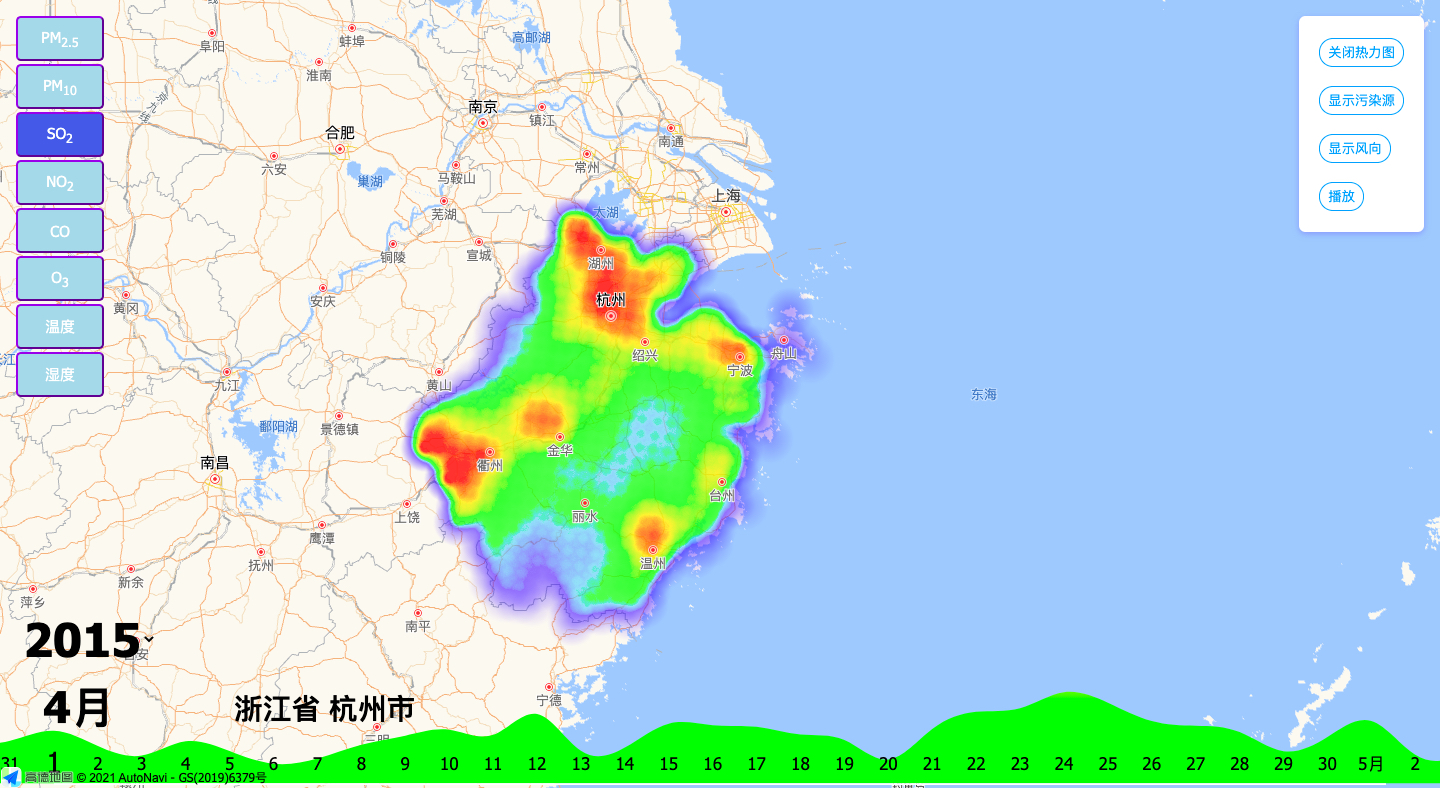
\includegraphics[width=0.5\columnwidth]{images/time_space10.png}}
        \caption{浙江省污染局部热力图}
        \label{fig:time_space2}
    \end{figure}

    \subsection{大气污染传输模式分析}
    % 利用可视分析技术,比较各地大气污染物差异、大气污染传输模式、检测异常传输事件,制定传输防治策略。
    % TODO: 陈雪韬
	% 343 字    
    
    \begin{figure}[h!]
        \centering
        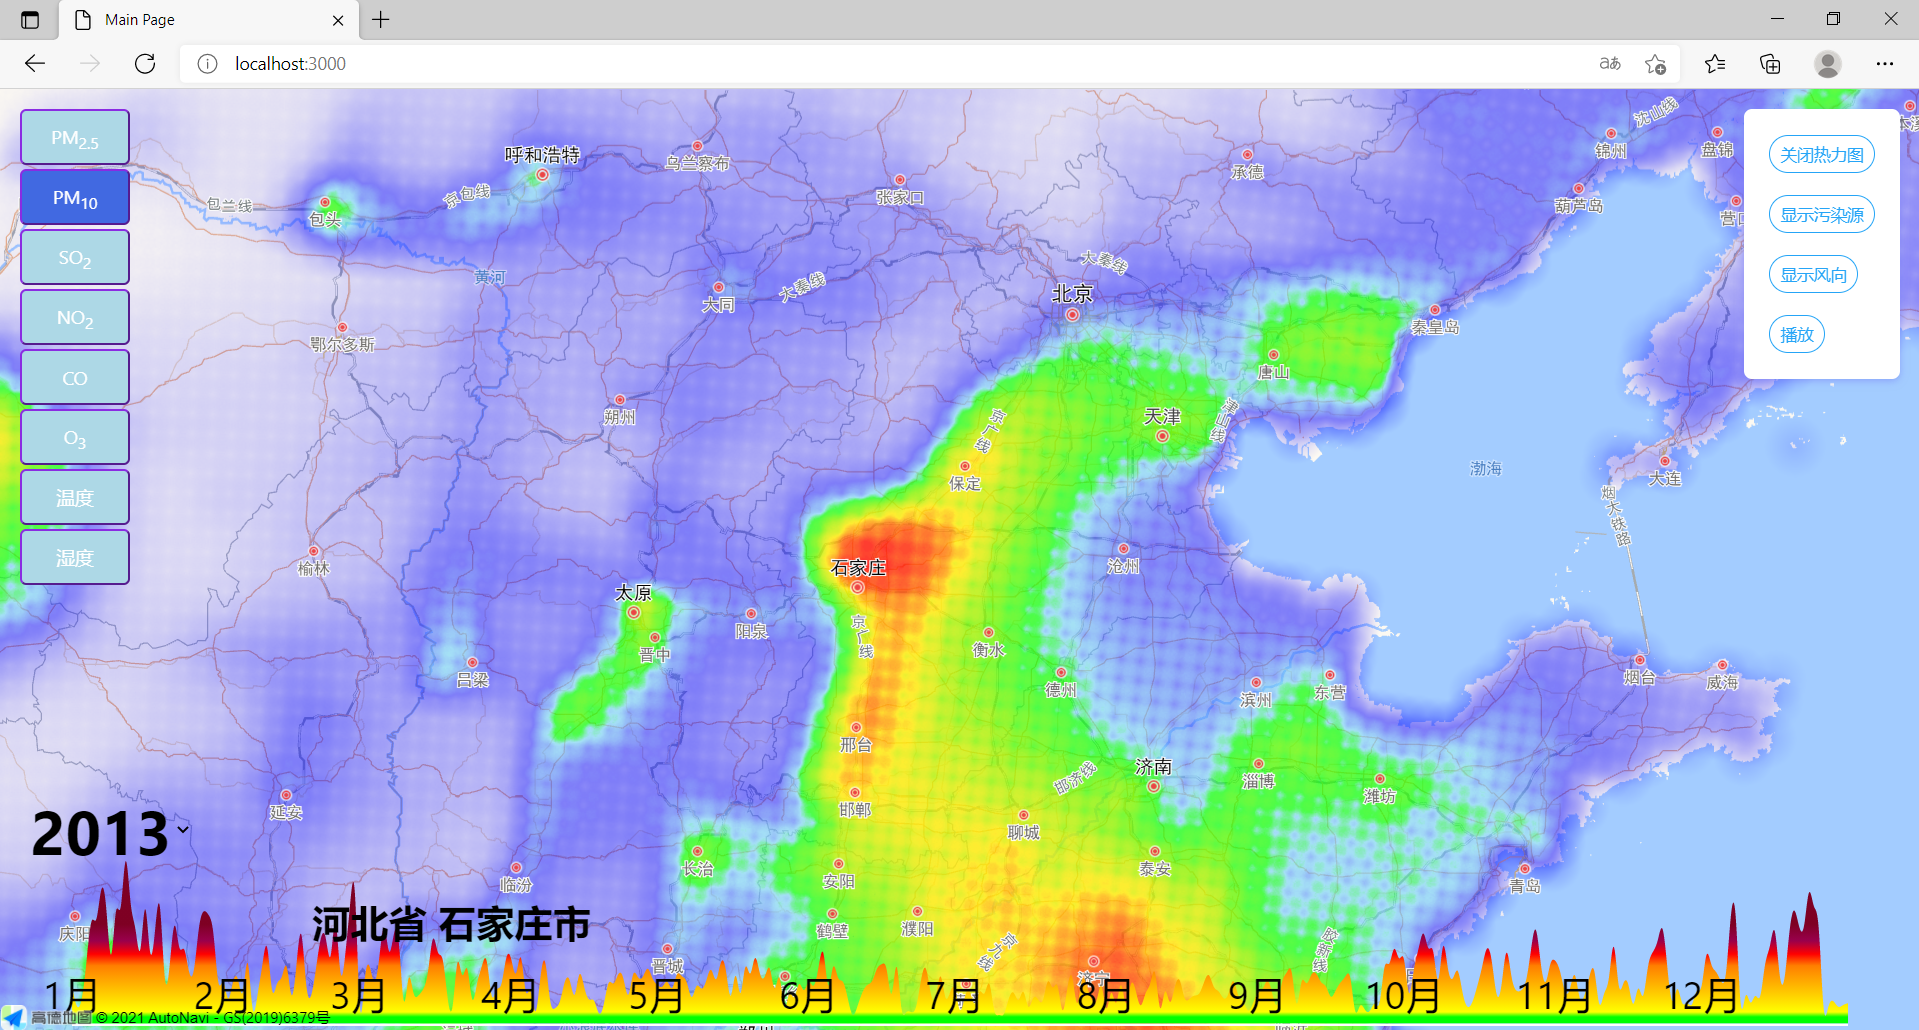
\includegraphics[width=15cm,keepaspectratio]{images/shijiazhuang_2013PM10.png}
        \caption{石家庄 2013 年 $\mathrm{PM}_{10}$ 污染图}
        \label{fig:shijiazhuang_2013PM10}
    \end{figure}
    石家庄是 $\mathrm{PM}_{10}$ 污染较为严重的一地。通过对石家庄当地的 $\mathrm{PM}_{10}$ 均值图(图 \ref{fig:shijiazhuang_2013PM10})的查看,可以发现石家庄在冬季的污染要远远大于其他季节。
    \par
    打开风向图,我们可以查看石家庄当地盛行的风向。选择石家庄冬季时间,点击播放按钮,连续观察石家庄的风向变化。可以看到,当西风较为强盛时,石家庄城市中的风力却一般都很小或者接近零,这是导致石家庄内部污染物不能够很好扩散的原因,而石家庄冬季盛行西北风(图 \ref{fig:shijiazhuang_wind1})。
	\par    
    查看地形图可知,石家庄西倚太行山脉,山脉阻挡了西北风吹过石家庄主城区,造成了石家庄冬季污染易积聚不能扩散,从而较夏季严重的特征;而石家庄冬季盛行的西北风是由西伯利亚冷高压在我国大多数地区引起的。
    \par 
    针对石家庄在冬季污染物扩散较为艰难的特点,石家庄要在冬季对污染物排放进行限制,并尤为注意风向对于污染物扩散的影响。\\
    \begin{figure}[h!]
        \centering
        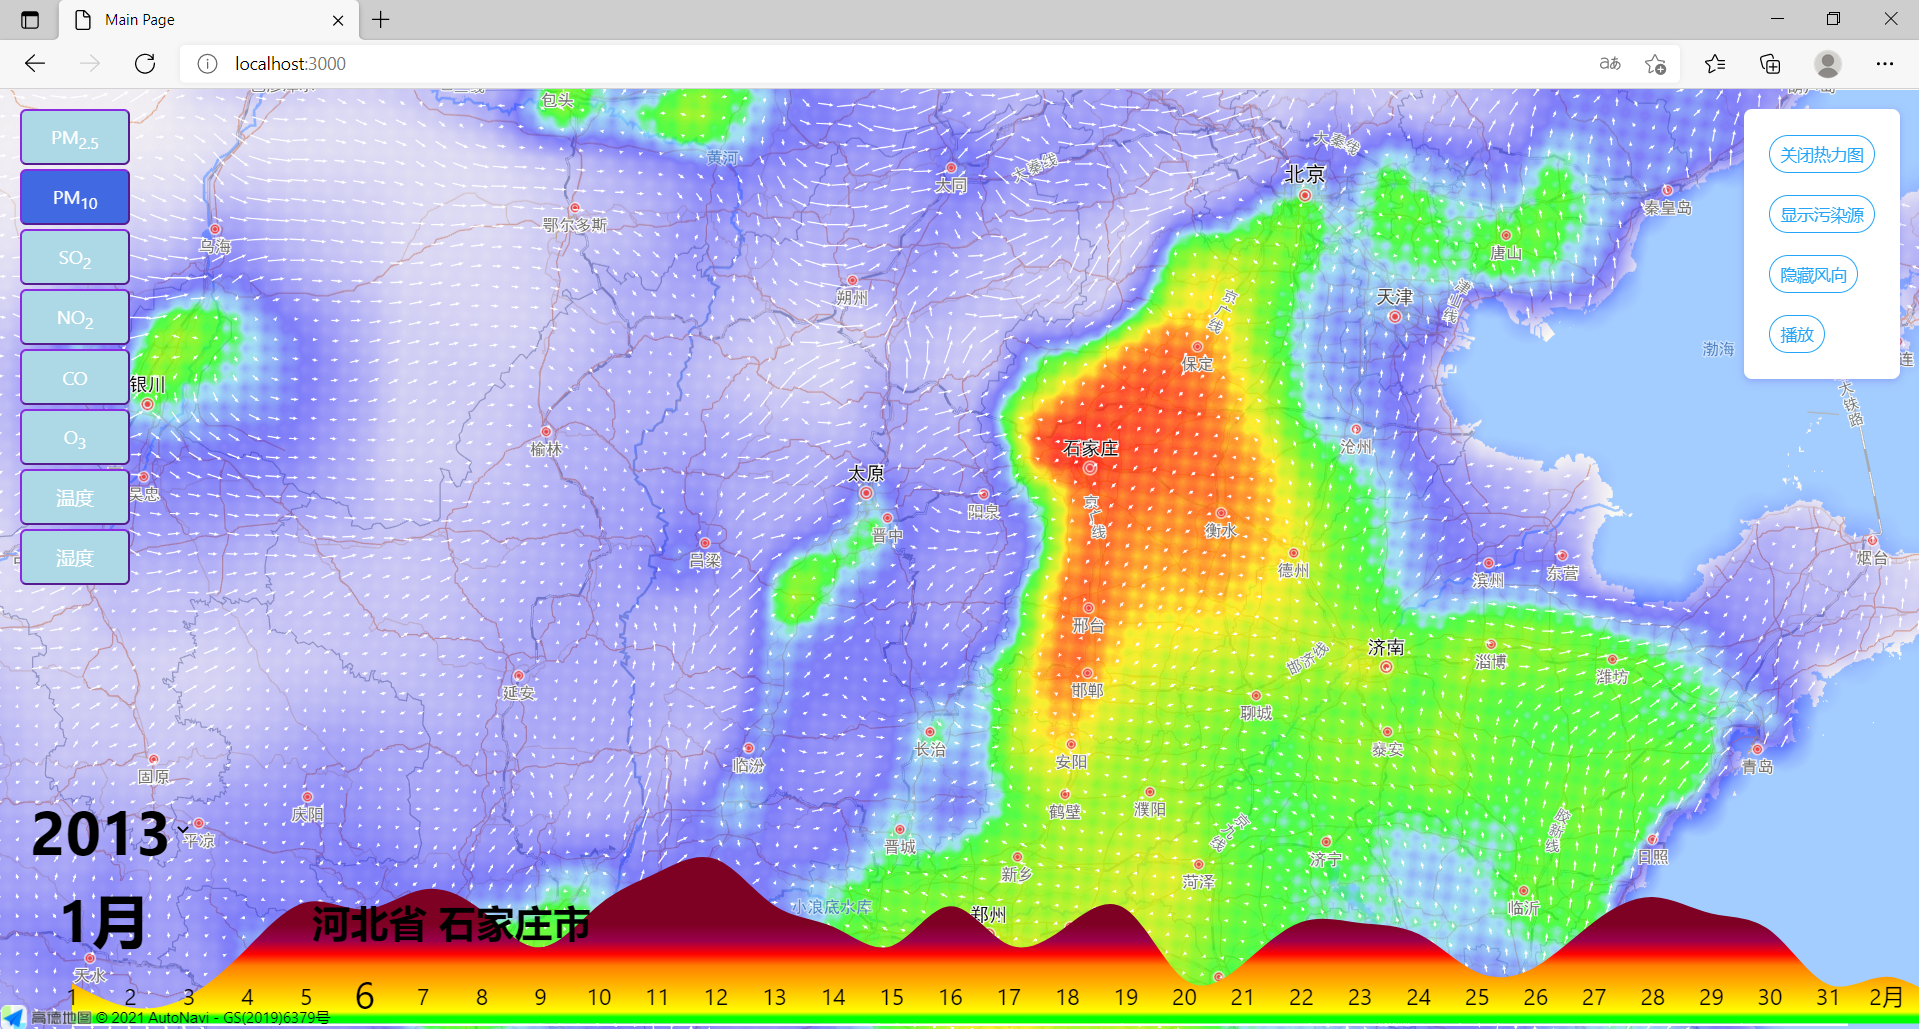
\includegraphics[width=15cm,keepaspectratio]{images/shijiazhuang_wind1.png}
        \caption{石家庄 2013 年 1 月 6 日 $\mathrm{PM}_{10}$ 污染分布}
        \label{fig:shijiazhuang_wind1}
    \end{figure}
    

    \subsection{大气环境的改善}
    % 利用可视分析技术,展示大气污染治理过程中的大气环境状况、评估大气污染防治措施。
    % TODO: 黄霖

    \section{讨论与总结}
    % (建议参赛者描述本部分内容不多于500字)
    % TODO: 方志成
    \subsection{讨论}
    \textbf{系统优化:}为了保证用户与界面交互的实时性,本项目采用了后端建立数据库,并通过NodeJS调用better-sqlite3库的方式降低数据传输的时延;此外,对于主界面的热力图,本项目组采用图层刷新的方式,实时创建最新图层并销毁旧图层,避免了资源的浪费,也使得前端操作更加顺滑。
    
    \textbf{数据阐释:}本系统侧重于2013-2018年历史污染数据的可视化展现,而并没有实时的2021数据呈现。但是,从历史数据的可视化中,使用者能够根据地图上的潜在污染源、风速风向情况以及时间信息,进行大气污染的综合分析,进而指定具备针对性的环保计划。
     
    ~\\ 
    \subsection{总结}
    本项目组的地图大屏很好地展示了各类污染源在各个地区随时间的变化情况,并通过热力图可以比较各个地区之间的污染情况。此外,风向图的加入有利于使用者进行季节性污染的分析;而创新性地将各地的工厂信息加入地图,更有利于相关部门进行污染源的追溯以及未来污染整治的规划。
    
    总体来看,本系统达到了最初的设计目标,可以被应用在气象局、环境局的污染分析部门中,辅助专业从事者进行大气污染分析。

\end{document}